% Immutable derivative of the approved representative sample.
% PDF pages 51--55 / printed pages 37--41; bytes below are copied without translation changes.
\setcounter{section}{2}
\section{向量场的分解}\label{sec:vector-field-decomposition}
在上一小节中得到正交子空间分解
\[
  L^2(\Omega)^N=H\oplus H^\perp,
  \qquad H_0^1(\Omega)^N=V\oplus V^\perp,
\]
并刻画了 $H^\perp$ 与 $V^\perp$. 这里将把 $H$ 和 $V$ 刻画为流函数的 curl 所成的空间.
特别地, 这将说明 $L^2(\Omega)^N$ 中每个函数都是一个流函数的 curl 与一个梯度之和.

\SampleSourcePage{51}{37}
\begin{figure}[htbp]
\centering
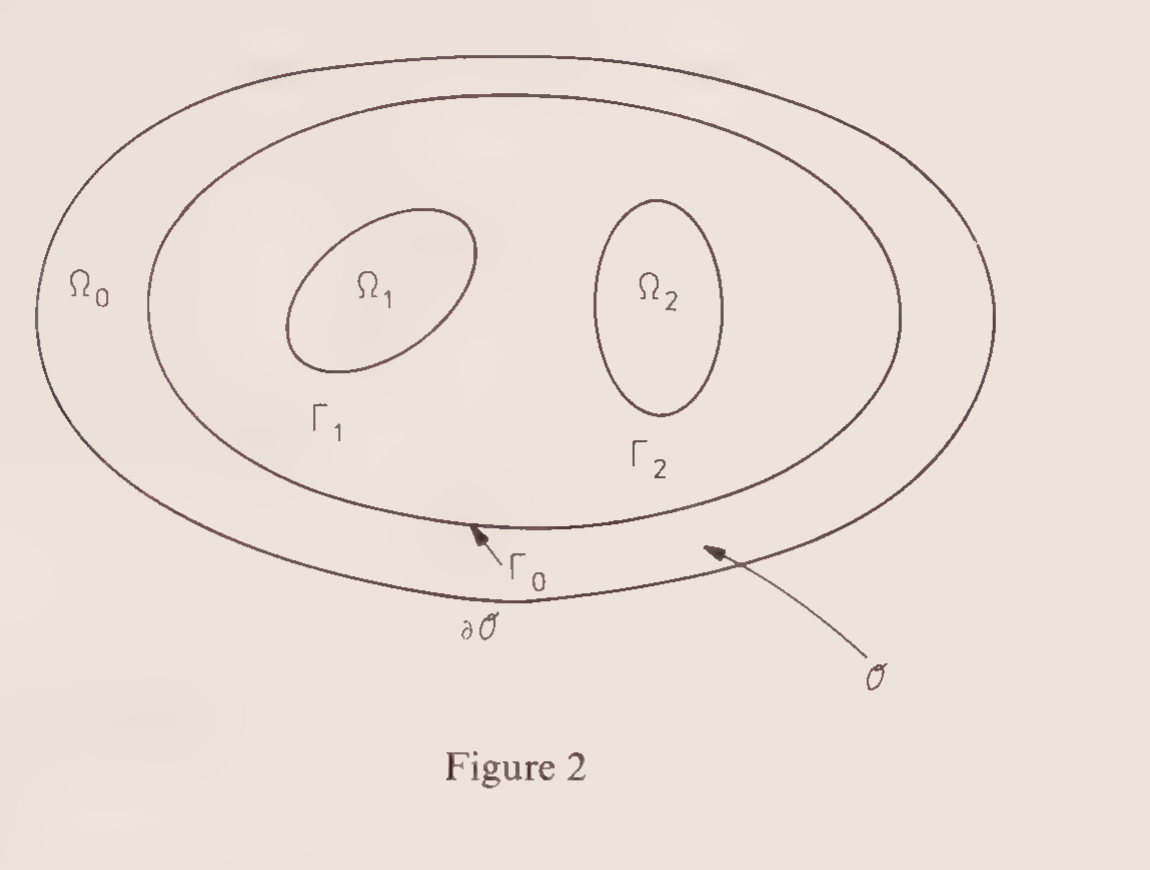
\includegraphics[width=.55\linewidth]{figures/figure-2.png}
\caption{多连通区域及其边界分支.}\label{fig:sec3-multiply-connected-domain}
\end{figure}
对 $\Omega$ 作如下假设: $\Omega$ 有界、连通但可以是多连通的, 其边界 $\Gamma$ Lipschitz 连续.
以 $\Gamma_0$ 表示 $\Omega$ 的外边界(见 Figure~\ref{fig:sec3-multiply-connected-domain}),
以 $\Gamma_i$, $1\le i\le p$, 表示 $\Gamma$ 的其他连通分支.
$H^{-1/2}(\Gamma_i)$ 与 $H^{1/2}(\Gamma_i)$ 之间的对偶记为
$\langle\cdot,\cdot\rangle_{\Gamma_i}$. 最后假设 $N=2$ 或 $N=3$.

\setcounter{subsection}{0}
\subsection{二维向量场的分解}\label{subsec:two-dimensional-decomposition}
\setcounter{statement}{0}
\setcounter{equation}{0}
\begin{Theorem}\label{thm:sec3-stream-function-characterization}
函数 $\mathbf v\in L^2(\Omega)^2$ 满足
\begin{equation}\label{eq:sec3-divfree-zero-flux}
  \Div\mathbf v=0,
  \qquad\langle\mathbf v\cdot\mathbf n,1\rangle_{\Gamma_i}=0
  \quad\text{for }0\le i\le p,
\end{equation}
当且仅当存在流函数 $\phi\in H^1(\Omega)$ 使得
\begin{equation}\label{eq:sec3-v-curl-phi}
  \mathbf v=\Curl\phi.
\end{equation}
\end{Theorem}
\begin{Proof}
1) 先证 \eqref{eq:sec3-v-curl-phi} 蕴含 \eqref{eq:sec3-divfree-zero-flux}.
令 $\phi\in H^1(\Omega)$ 并令 $\mathbf v=\Curl\phi$. 显然
$\Div\mathbf v=0$. 又因 $\D(\overline\Omega)$ 在 $H^1(\Omega)$ 中稠密,
只需证明
\[
  \int_{\Gamma_i}\Curl\phi\cdot\mathbf n\dd s=0
  \quad\forall\phi\in\D(\overline\Omega),\quad0\le i\le p.
\]
这确实成立, 因为
\[
  \int_{\Gamma_i}\Curl\phi\cdot\mathbf n\dd s
  =\int_{\Gamma_i}(\partial\phi/\partial\tau)\dd s=0.
\]

\SampleSourcePage{52}{38}
2) 反之, 设 $\mathbf v$ 满足 \eqref{eq:sec3-divfree-zero-flux}. 思路是将
$\mathbf v$ 延拓到整个平面且保持无散, 然后利用 Fourier 变换构造其流函数.

a) 使用一个在 $\Gamma$ 上与 $\mathbf v$ 具有相同法向分量的延拓.
取任意有界、光滑、单连通开集 $\mathcal O$, 使
$\overline\Omega\subset\mathcal O$. 当 $p\ge1$ 时,
$\mathcal O-\overline\Omega$ 不连通. 对 $1\le i\le p$, 以 $\Omega_i$ 表示由
$\Gamma_i$ 围成的连通分支; 以 $\Omega_0$ 表示由 $\Gamma_0$ 和
$\partial\mathcal O$ 围成的连通分支(见 Figure~\ref{fig:sec3-multiply-connected-domain}).
考虑问题: 求定义在 $\mathcal O-\overline\Omega$ 上的 $w$, 使
\[
\left\{\begin{aligned}
  \Delta w&=0&&\text{in }\mathcal O-\overline\Omega,\\
  \partial w/\partial n&=\mathbf v\cdot\mathbf n&&\text{on }\Gamma_i,
       \quad0\le i\le p,\\
  \partial w/\partial n&=0&&\text{on }\partial\mathcal O.
\end{aligned}\right.
\tag{N}
\]
其中 $\mathbf n$ 表示指向 $\Omega_i$ 外部的 $\Gamma_i$ 上单位法向量.
问题 $(N)$ 由 $p+1$ 个非齐次 Neumann 问题组成, 每个定义在
$\Omega_i$, $0\le i\le p$, 上; 它们如同
Section~\ref{sec:abstract-variational-problem} 中分析的问题, 因为都满足相容条件
\[
  \langle\mathbf v\cdot\mathbf n,1\rangle_{\Gamma_i}=0
  \quad\text{for }0\le i\le p.
\]
因此存在 $w\in H^1(\mathcal O-\overline\Omega)$ 满足 $(N)$, 且在每个
$\Omega_i$ 中相差一个加性常数的意义下唯一. 令
\[
  \boldsymbol\theta=\Grad w.
\]
则 $\boldsymbol\theta\in H(\Div;\mathcal O-\overline\Omega)$, 并满足
\begin{equation}\label{eq:sec3-extension-normal-data}
\left\{\begin{aligned}
  \Div\boldsymbol\theta&=\Delta w=0&&\text{in }\mathcal O-\overline\Omega,\\
  \boldsymbol\theta\cdot\mathbf n&=\partial w/\partial n
    =\mathbf v\cdot\mathbf n&&\text{on }\Gamma_i,
      \quad0\le i\le p,\\
  \boldsymbol\theta\cdot\mathbf n&=0&&\text{on }\partial\mathcal O.
\end{aligned}\right.
\end{equation}

b) 现在把 $\mathbf v$ 延拓为
\[
  \widetilde{\mathbf v}=\begin{cases}
  \mathbf v,&\text{in }\Omega,\\
  \boldsymbol\theta,&\text{in }\mathcal O-\Omega,\\
  0,&\text{elsewhere}.
  \end{cases}
\]
显然 $\widetilde{\mathbf v}\in L^2(\R^2)^2$. 作为分布, 它的散度满足
\[
  \langle\Div\widetilde{\mathbf v},\phi\rangle
  =-\int_{\R^2}\widetilde{\mathbf v}\cdot\Grad\phi\dd x
  \quad\forall\phi\in\D(\R^2),
\]
即
\[
  \langle\Div\widetilde{\mathbf v},\phi\rangle
  =-\int_\Omega\mathbf v\cdot\Grad\phi\dd x
  -\sum_{i=0}^{p}\int_{\Omega_i}\boldsymbol\theta\cdot\Grad\phi\dd x.
\]
由于 $\mathbf v$ 与 $\boldsymbol\theta$ 都无散, 由 Green 公式
\eqref{eq:sec2-hdiv-green} 和 \eqref{eq:sec3-extension-normal-data} 得到

\SampleSourcePage{53}{39}
\[
  \langle\Div\widetilde{\mathbf v},\phi\rangle
  =-\langle\mathbf v\cdot\mathbf n,\phi\rangle_\Gamma
  -\sum_{i=0}^{p}\langle\mathbf v\cdot\mathbf n,\phi\rangle_{\Gamma_i}.
\]
上式求和中的 $\Gamma_i$ 法向量指向 $\Omega_i$ 外部, 因而指向 $\Omega$ 内部;
所以和式中的每一项都与 $\langle\mathbf v\cdot\mathbf n,\phi\rangle_\Gamma$
中的一项相消. 因此
\[
  \langle\Div\widetilde{\mathbf v},\phi\rangle=0
  \quad\forall\phi\in\D(\R^2),
\]
即 $\Div\widetilde{\mathbf v}=0$.

c) 因 $\widetilde{\mathbf v}$ 的支集紧, 由 \eqref{eq:sec2-fourier-transform-vector}
定义的 Fourier 变换 $\mathcal F\widetilde{\mathbf v}$ 是关于 $\boldsymbol\mu$ 的全纯函数.
用 Fourier 变换表示 $\Div\widetilde{\mathbf v}=0$ 与
$\widetilde{\mathbf v}=\Curl\phi$, 得
\begin{equation}\label{eq:sec3-fourier-divfree}
  \mu_1\mathcal F\widetilde v_1+
  \mu_2\mathcal F\widetilde v_2=0,
\end{equation}
\begin{equation}\label{eq:sec3-fourier-stream}
  \mathcal F\widetilde v_1=2i\pi\mu_2\mathcal F\phi,
  \qquad
  \mathcal F\widetilde v_2=-2i\pi\mu_1\mathcal F\phi.
\end{equation}
若取 $\mathcal F\phi=\mathcal F\widetilde v_1/(2i\pi\mu_2)$, 则由
\eqref{eq:sec3-fourier-divfree}, \eqref{eq:sec3-fourier-stream} 的两个等式都成立, 即
\[
  \mathcal F\phi=\frac{\mathcal F\widetilde v_1}{2i\pi\mu_2}
  =-\frac{\mathcal F\widetilde v_2}{2i\pi\mu_1}.
\]
因此, 只要 $\mathcal F\phi\in L^2(\R^2)$, 它的逆变换就是
$\widetilde{\mathbf v}$ 所需的流函数. 由于
$\mathcal F\widetilde v_i\in L^2(\R^2)$, 只需证明
$\mathcal F\phi$ 在原点邻域内有界.

由 \eqref{eq:sec3-fourier-divfree}, 有
$\mathcal F\widetilde v_1(\mu_1,0)=0$. 利用
$\mathcal F\widetilde v_1$ 的全纯性得到
\[
  \mathcal F\widetilde v_1(\mu_1,\mu_2)
  =\mu_2\frac{\partial\mathcal F\widetilde v_1(\mu_1,0)}{\partial\mu_2}
  +O(|\mu_2|^2),
\]
从而
\[
  \mathcal F\phi(\mu_1,\mu_2)
  =\frac1{2i\pi}\frac{\partial\mathcal F\widetilde v_1(\mu_1,0)}{\partial\mu_2}
  +O(|\mu_2|).
\]
显然这说明 $\mathcal F\phi$ 在原点邻域内有界.
\end{Proof}

该定理的一个直接推论是: 若 $\mathbf v\in L^s(\Omega)^2$ 对某个实数
$s\ge2$ 成立(相应地, $\mathbf v\in H^m(\Omega)^2$ 对某个整数 $m\ge0$ 成立),
且 $\mathbf v$ 满足 $\Div\mathbf v=0$ 和
$\langle\mathbf v\cdot\mathbf n,1\rangle_{\Gamma_i}=0$, $0\le i\le p$, 则
\[
  \mathbf v=\Curl\phi,
  \quad \phi\in W^{1,s}(\Omega)
  \quad(\text{相应地 }\phi\in H^{m+1}(\Omega)).
\]
注意到 $\Omega$ 连通, $\mathbf v$ 的流函数 $\phi$ 在相差加性常数的意义下唯一.
特别地, 当 $\mathbf v\in H$ 时, 其流函数满足
$(\partial\phi/\partial\tau)|_{\Gamma_i}=0$, 即
\[
  \phi|_{\Gamma_i}=\text{常数 }c_i,
  \quad0\le i\le p.
\]
因此固定这些常数中的一个后, $\phi$ 唯一确定. 例如, $\mathbf v$ 恰有一个在
$\Gamma_0$ 上为零的流函数 $\phi$. 该函数属于下列空间.

\SampleSourcePage{54}{40}
\begin{equation}\label{eq:sec3-phi-space}
  \Phi=\{\chi\in H^1(\Omega);\ \chi|_{\Gamma_0}=0,
  \ \chi|_{\Gamma_i}=\text{任意常数},\ 1\le i\le p\}.
\end{equation}
这是 $H^1(\Omega)$ 的闭子空间. 此外, 由下面的 Poincaré
Theorem~\ref{thm:poincare-friedrichs} 的推广,
$|\cdot|_{1,\Omega}$ 与 $\|\cdot\|_{1,\Omega}$ 是 $\Phi$ 上的两个等价范数.
该结论的证明可由 Theorem~\ref{thm:peetre-tartar-compact-operator} 的 $2^\circ)$ 直接得到.

\setcounter{statement}{0}
\begin{Lemma}\label{lem:sec3-boundary-poincare}
设 $\Gamma_0$ 是 $\Gamma$ 中测度严格为正的一部分. 则对任意实数 $r\ge1$,
$|\cdot|_{1,r,\Omega}$ 与 $\|\cdot\|_{1,r,\Omega}$ 是空间
\[
  \{v\in W^{1,r}(\Omega);\ v|_{\Gamma_0}=0\}
\]
上的两个等价范数.
\end{Lemma}

下一个推论把属于 $\Phi$ 的特殊流函数刻画为边值问题的解. 它直接由
Theorem~\ref{thm:sec3-stream-function-characterization} 和
Lemma~\ref{lem:sec3-boundary-poincare} 得到.

\setcounter{statement}{0}
\begin{Corollary}\label{cor:sec3-h-stream-functions}
空间 $H$ 有如下刻画:
\[
  H=\{\Curl\phi;\ \phi\in\Phi\},
\]
且映射 $\Curl$ 是从 $\Phi$ 到 $H$ 的同构. 此外, $\mathbf v$ 的流函数
$\phi$ 是问题
\begin{equation}\label{eq:sec3-stream-variational}
  \phi\in\Phi,
  \qquad(\Curl\phi,\Curl\chi)=(\mathbf v,\Curl\chi)
  \quad\forall\chi\in\Phi
\end{equation}
的唯一解.
\end{Corollary}

\setcounter{statement}{0}
\begin{Remark}\label{rem:sec3-stream-boundary-problem}
问题 \eqref{eq:sec3-stream-variational} 可解释为
\[
\left\{\begin{aligned}
  -\Delta\phi&=\Curl\mathbf v&&\text{in }\D'(\Omega),\\
  \phi|_{\Gamma_0}&=0,\qquad \phi|_{\Gamma_i}=c_i,\\
  \langle\partial\phi/\partial n+\mathbf v\cdot\boldsymbol\tau,1\rangle_{\Gamma_i}
    &=0&&1\le i\le p.
\end{aligned}\right.
\]
第一式由取测试函数 $\chi\in\D(\Omega)$ 得到. 为推出 $\Gamma_i$ 上最后一个边界条件,
注意到 \eqref{eq:sec2-laplace-green} 形式上给出
\[
  (\Curl\phi,\Curl\chi)=-(\Delta\phi,\chi)
  +\langle\partial\phi/\partial n,\chi\rangle_\Gamma
  \quad\forall\chi\in H^1(\Omega).
\]
同样, \eqref{eq:sec2-hcurl-green} 形式上给出
\[
  (\mathbf v,\Curl\chi)=(\Curl\mathbf v,\chi)
  -\langle\mathbf v\cdot\boldsymbol\tau,\chi\rangle_\Gamma
  \quad\forall\chi\in H^1(\Omega).
\]
将这两个等式与 \eqref{eq:sec3-stream-variational} 比较, 得
\[
  \sum_{i=1}^{p}
  \langle\partial\phi/\partial n+\mathbf v\cdot\boldsymbol\tau,c_i\rangle_{\Gamma_i}=0
  \quad\forall c_i\in\R.
\]
\end{Remark}

Theorem~\ref{thm:sec3-stream-function-characterization} 及其推论给出
$L^2(\Omega)^2$ 的如下正交分解.

\setcounter{statement}{1}
\begin{Theorem}\label{thm:sec3-orthogonal-decomposition}
$L^2(\Omega)^2$ 中每个函数 $\mathbf v$ 都有如下正交分解:
\begin{equation}\label{eq:sec3-orthogonal-decomposition}
  \mathbf v=\Grad q+\Curl\phi,
\end{equation}
其中 $q\in H^1(\Omega)/\R$ 是问题
\begin{equation}\label{eq:sec3-neumann-variational}
  (\Grad q,\Grad\mu)=(\mathbf v,\Grad\mu)
  \quad\forall\mu\in H^1(\Omega)
\end{equation}
的唯一解, 而 $\phi\in\Phi$ 是问题
\begin{equation}\label{eq:sec3-curl-remainder-variational}
  (\Curl\phi,\Curl\chi)=(\mathbf v-\Grad q,\Curl\chi)
  \quad\forall\chi\in\Phi
\end{equation}
的唯一解.
\end{Theorem}

\SampleSourcePage{55}{41}
\begin{Proof}
对 $\mathbf v\in L^2(\Omega)^2$, Neumann 问题
\eqref{eq:sec3-neumann-variational} 在 $H^1(\Omega)/\R$ 中有唯一解 $q$.
该解满足
\[
  \Delta q=\Div\mathbf v\quad\text{in }H^{-1}(\Omega).
\]
所以 $\mathbf v-\Grad q$ 是 $H(\Div;\Omega)$ 中的无散向量. 此外, 把 Green 公式
\eqref{eq:sec2-hdiv-green} 应用于 \eqref{eq:sec3-neumann-variational}, 得
\[
  0=(\mathbf v-\Grad q,\Grad\mu)
  =\langle(\mathbf v-\Grad q)\cdot\mathbf n,\mu\rangle_\Gamma
  \quad\forall\mu\in H^1(\Omega),
\]
故 $(\mathbf v-\Grad q)\cdot\mathbf n=0$ in $H^{-1/2}(\Gamma)$.
换言之, $\mathbf v-\Grad q\in H$. 由 Corollary~\ref{cor:sec3-h-stream-functions},
存在唯一 $\phi\in\Phi$ 满足 \eqref{eq:sec3-orthogonal-decomposition} 和
\eqref{eq:sec3-curl-remainder-variational}.
\end{Proof}

\setcounter{statement}{1}
\begin{Remark}\label{rem:sec3-neumann-interpretation}
当 $\mathbf v\in H(\Div;\Omega)$ 时, 问题 \eqref{eq:sec3-neumann-variational}
可解释为
\[
\left\{\begin{aligned}
  \Delta q&=\Div\mathbf v&&\text{in }\Omega,\\
  \partial q/\partial n&=\mathbf v\cdot\mathbf n&&\text{on }\Gamma.
\end{aligned}\right.
\]
若 $\mathbf v$ 仅属于 $L^2(\Omega)^2$, 最后一个等式只是形式上的.
\end{Remark}

本节的方法可以直接把 Lemma~\ref{lem:sec2-div-free-lifting} 推广到更光滑的函数.

\setcounter{statement}{1}
\begin{Lemma}\label{lem:sec3-smooth-divfree-lifting}
设 $\Omega$ 是 $\R^2$ 中的有界连通区域, 边界 $\Gamma$ 属于
$\mathcal C^{m,1}$ 类($m\ge2$), 且
$\mathbf g\in H^{m-1/2}(\Gamma)^2$ 满足
\[
  \int_\Gamma\mathbf g\cdot\mathbf n\dd s=0.
\]
则存在 $\mathbf u=f(\mathbf g)\in H^m(\Omega)^2$ 使得
\[
  \Div\mathbf u=0\quad\text{in }\Omega,
  \qquad\mathbf u=\mathbf g\quad\text{on }\Gamma,
\]
并且
\[
  \|\mathbf u\|_{m,\Omega}\le C\|\mathbf g\|_{m-1/2,\Gamma}.
\]
\end{Lemma}
\begin{Proof}
这里只勾勒证明. 边界条件 $\mathbf u=\mathbf g$ on $\Gamma$ 可分解为
$\mathbf u\cdot\mathbf n=\mathbf g\cdot\mathbf n$ 和
$\mathbf u\cdot\boldsymbol\tau=\mathbf g\cdot\boldsymbol\tau$ on $\Gamma$.
分别指定这两个条件较为简单, 因而设
\[
  \mathbf u=\Grad q+\Curl\phi.
\]
% Proof continues on PDF page 56 / printed page 42.
